%
%
%

%%%%%%%%%%%%%%%%%%%%%%%%%%%%%%%%%%%%%%%%%%%%%%%%%%%%%%%%%%%%%%%%%%%%%%%%
% Exercise
%
\exercises

\begin{exercise}{files1}
Consider a file \hbox{\lstinline+f.ml+} with the following contents.
\begin{ocaml}
type t = int
let f x = x
\end{ocaml}
%
Which of the following are legal \hbox{\lstinline+f.mli+} files?

\begin{enumerate}
\item \lstinline+f.mli+ is empty.

\item \lstinline+f.mli+:
\begin{ocaml}
val f : 'a -> 'a
\end{ocaml}

\item \lstinline+f.mli+:
\begin{ocaml}
val f : ('a -> 'b) -> ('a -> 'b)
\end{ocaml}

\item \lstinline+f.mli+:
\begin{ocaml}
val f : t -> t
\end{ocaml}

\item \lstinline+f.mli+:
\begin{ocaml}
type t
val f : t -> t
\end{ocaml}

\item \lstinline+f.mli+:
\begin{ocaml}
type s = int
val f : s -> s
\end{ocaml}
\end{enumerate}

\begin{answer}\ifanswers
\begin{enumerate}
\item

It is always legal for a \hbox{\lstinline+.mli+} file to be empty.
However, this hides all definitions in the \hbox{\lstinline+.ml+}
file, so it has limited usefulness.

\item

The specification \hbox{\lstinline+val f : 'a -> 'a+} is legal.

\item

The specification \hbox{\lstinline+val f : ('a -> 'b) -> ('a -> 'b)+}
is also legal (it is just a refinement of the type
\hbox{\lstinline+'a -> 'a+}).

\item 

The specification \hbox{\lstinline+val f : t -> t+} is not legal
because there is no definition for the type \hbox{\lstinline+t+}.

\item

The specification \hbox{\lstinline+type t val f : t -> t+} is legal.

\item

The specification \hbox{\lstinline+type s = int val f : s -> s+} is
not legal because the type \hbox{\lstinline+s+} must also be defined
in the \hbox{\lstinline+.ml+} file.
\end{enumerate}
\fi\end{answer}
\end{exercise}

%%%%%%%%%%%%%%%%%%%%%%%%%%%%%%%%%%%%%%%%%%%%%%%%%%%%%%%%%%%%%%%%%%%%%%%%
% Exercise
%
\begin{exercise}{hide1}
Consider the following two versions of a list reversal function.

\begin{center}
\begin{tabular}{ll}
\begin{tabular}{l}
rev.mli\\
\hline
\begin{ocaml}
val rev : 'a list -> 'a list
\end{ocaml}
\end{tabular}
\\
\\
\begin{tabular}[t]{l}
rev.ml (version 1)\\
\hline
\begin{minipage}{2in}
\begin{ocamllisting}
let rev l =
   let rec rev_loop l1 l2 =
      match l2 with
         x :: l2 ->
            loop (x :: l1) l2
       | [] ->
            l1
   in
      rev_loop [] l
\end{ocamllisting}
\end{minipage}
\end{tabular}
&
\begin{tabular}[t]{l}
rev.ml (version 2)\\
\hline
\begin{minipage}{2in}
\begin{ocamllisting}
let rec rev_loop l1 l2 =
   match l2 with
      x :: l2 ->
         loop (x :: l1) l2
    | [] ->
         l1

let rev l = rev_loop [] l
\end{ocamllisting}
\end{minipage}
\end{tabular}
\end{tabular}
\end{center}
%
\begin{enumerate}
\item Is there any reason to prefer one version over the other?
\item
In the second version, what would happen if we defined
the \hbox{\lstinline+rev+} function as a partial application?
%
\begin{ocaml}
(* let rev l = rev_loop [] l *)
let rev = rev_loop []
\end{ocaml}
\end{enumerate}

\begin{answer}\ifanswers
\begin{enumerate}
\item

There are differences, but it isn't clear that one version is better
than the other.  In version 1, the variable \hbox{\lstinline+l+} is
bound (and visible) in the \hbox{\lstinline+rev_loop+} function.  Some
typographical errors (for example, if we had
written \hbox{\lstinline+match l with ...+} instead
of \hbox{\lstinline+match l2 with ...+}) will not be caught at compile
time.

Version 2 has a similar problem; the \hbox{\lstinline+rev_loop+}
function is visible in the rest of the file, so it might be used
accidentally.  Note however, that the
signature \hbox{\lstinline+rev.mli+} hides the definition from the
rest of the program.

\item

The partial application \hbox{\lstinline+let rev = rev_loop []+} is
not allowed, as it has type \hbox{\lstinline+'_a -> '_a+},
not \hbox{\lstinline+'a -> 'a+}.  See
Section~\ref{section:value-restriction}, which discusses the value
restriction.

\end{enumerate}
\fi\end{answer}
\end{exercise}

%%%%%%%%%%%%%%%%%%%%%%%%%%%%%%%%%%%%%%%%%%%%%%%%%%%%%%%%%%%%%%%%%%%%%%%%
% Exercise
%
\begin{exercise}{infer1}
\index{interfaces!automatically generating}
When a program is begin developed, it is sometimes convenient to have the
compiler produce a \hbox{\lstinline+.mli+} file automatically, using
the \hbox{\lstinline+-i+} option to \hbox{\lstinline+ocamlc+}.  For
example, suppose we have an implementation
file \hbox{\lstinline+set.ml+} containing the following definitions.

\begin{ocaml}
type 'a set = 'a list
let empty = []
let add x s = x :: s
let mem x s = List.mem x s
\end{ocaml}
%
Inferring types, we obtain the following output.  The output can then
be edited to produce the desired \hbox{\lstinline+set.mli+} file.
\begin{ocaml}
% ocamlc -i set.ml
type 'a set = 'a list
val empty : 'a list
val add : 'a -> 'a list -> 'a list
val mem : 'a -> 'a list -> bool
\end{ocaml}

\begin{enumerate}
\item

The output produced by \hbox{\lstinline+ocamlc -i+} is not abstract---the
declarations use the type
%
\hbox{\lstinline+'a list+},
%
not \hbox{\lstinline+'a set+}.  Instead of editing all the occurrences by hand, is
there a way to get \hbox{\lstinline+ocamlc -i+} to produce the right output
automatically?

\item

In some cases, \hbox{\lstinline+ocamlc -i+} produces illegal output.
What is the inferred interface for the following program?  What is
wrong with it?  Can it be fixed?

\begin{ocaml}
let cell = ref []
let push i = cell := i :: !cell
let pop () =
   match !cell with
      [] -> raise (Invalid_argument "pop")
    | i :: t ->
        cell := t;
        i
\end{ocaml}
\end{enumerate}

\begin{answer}\ifanswers
\begin{enumerate}
\item

One solution is to add explicit type constraints to the source
program.  For example, if we revise the definition
for \hbox{\lstinline+add+} as follows, the correct type for it will be
inferred.
\begin{ocaml}
let add x (s : 'a set) : 'a set = x :: s
\end{ocaml}

\item The inferred type for this program is the following.

\begin{ocaml}
val cell : '_a list ref
val push : '_a -> unit
val pop : unit -> '_a
\end{ocaml}
%
Syntactically, the problem with this signature is the type
variable \hbox{\lstinline+'_a+}, which is not allowed in an interface
file.  The real problem is that the type of the reference cell is
unspecified, but it can only be used with one type.  To fix the
signature, we must choose a specific type for the stack.  For example,
the following is a valid signature that specifies that the stack is a
stack of integers.

\begin{ocaml}
val push : int -> unit
val pop : unit -> int
\end{ocaml}
\end{enumerate}
\fi\end{answer}
\end{exercise}

%%%%%%%%%%%%%%%%%%%%%%%%%%%%%%%%%%%%%%%%%%%%%%%%%%%%%%%%%%%%%%%%%%%%%%%%
% Exercise
%
\begin{exercise}{files3}
One issue we discussed was the need for duplicate type definitions.
If a \hbox{\lstinline+.mli+} provides a definition for a type \hbox{\lstinline+t+}, the the
\hbox{\lstinline+.ml+} file must specify exactly the same definition.  This can be
annoying if the type definition is to be changed.

One solution we discussed is to place the type definition in a
separate file, like \hbox{\lstinline+types.ml+}, with no interface file
\hbox{\lstinline+types.mli+}.  It is also legal to place the type definition in a
file \hbox{\lstinline+types.mli+} with no implementation \hbox{\lstinline+types.ml+}.

Is it ever preferable to use the second form (where \hbox{\lstinline+types.mli+}
exists, but \hbox{\lstinline+types.ml+} doesn't)?

\begin{answer}\ifanswers
The differences between the two include the following.
\begin{itemize}
\item

A \hbox{\lstinline+.mli+} file contains only declarations and type
definitions.  If the file contains a expression definition
(like \hbox{\lstinline+let zero = 0+}), then it must be placed in
a \hbox{\lstinline+.ml+} file.

\item

Components with only a \hbox{\lstinline+.mli+} file need not be
specified during linking.  This is a slight benefit, but it can
slightly simplify program construction in some cases.
\end{itemize}
\fi\end{answer}
\end{exercise}

%%%%%%%%%%%%%%%%%%%%%%%%%%%%%%%%%%%%%%%%%%%%%%%%%%%%%%%%%%%%%%%%%%%%%%%%
% Exercise
%
\begin{exercise}{files4}
The strict-ordering requirement during linking can potentially have a
major effect on the software design.  For example, suppose we were
designing a bi-directional communication protocol, as shown in the
following diagram.

\begin{center}
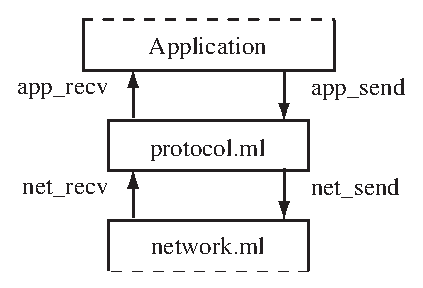
\includegraphics{network_stack}
\end{center}
%
With this design, the \hbox{\lstinline+Network+} component
calls \hbox{\lstinline+Protocol.net_recv+} when a message arrives, and
the \hbox{\lstinline+Protocol+} component
calls \hbox{\lstinline+Network.net_send+} to send a message.  However,
this is not possible if the implementations are in separate
files \hbox{\lstinline+protocol.ml+} and \hbox{\lstinline+network.ml+}
because that would introduce a cyclic dependency.

Describe a method to circumvent this problem, without placing the code
for the two components into a single file.

\begin{answer}\ifanswers
There are a few potential solutions, including the use of recursive
modules (discussed in Section~\ref{section:recursive-modules}) or
objects (Chapter~\ref{chapter:objects}).  In addition here are a few
alternate ways.

\begin{enumerate}
\item

If the design can be partitioned into two separate message streams
without any cycles, the design can be programmed directly.

\begin{center}
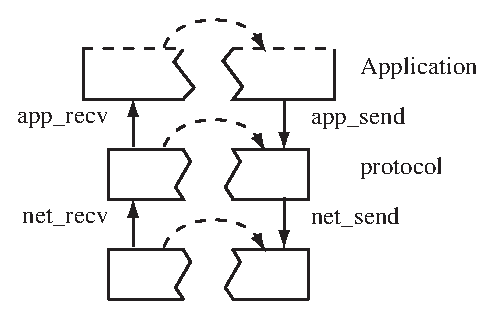
\includegraphics{network_stack2}
\end{center}
%
However, this approach may not be possible, and the changes required
may be unnatural.

\item

A simpler solution is to introduce a third file containing references
that can be set to refer each of the functions.  This solution, while
lacking elegance, is straightforward.

\begin{center}
\begin{tabular}{l}
refs.mli\\
\hline
\begin{minipage}{5in}
\begin{ocaml}
val net_recv_ref : (message -> unit) ref
val net_send_ref : (message -> unit) ref
val app_recv_ref : (message -> unit) ref
val app_send_ref : (message -> unit) ref
\end{ocaml}
\end{minipage}
\end{tabular}
\end{center}
%
The cells are initialized with dummy values.
\begin{ocaml}
let net_recv_ref = ref (fun _ -> raise (Invalid_argument "not initialized"))
...
\end{ocaml}
%
At startup time, the layers set the references to refer to the
appropriate functions.

\begin{center}
\begin{tabular}{l}
protocol.ml\\
\hline
\begin{minipage}{3in}
\begin{ocaml}
let net_recv msg = ...
...
Refs.net_recv_ref := net_recv
\end{ocaml}
\end{minipage}
\end{tabular}
\end{center}

\item

Yet another option is to define a third file,
say \hbox{\lstinline+link.ml+} that builds the recursive definition in
a single file.  Each of the layer functions would take as arguments
the functions that it expects to call.

\begin{ocaml}
let rec net_recv msg =
   Protocol.net_recv net_send app_recv msg
and app_send msg =
   Protocol.app_send net_send app_recv msg
and net_send msg =
   Network.net_send net_recv msg
and app_recv msg =
   Application.app_recv app_send msg
\end{ocaml}
%
This solution is more complicated and may be slightly less efficient
than the solution using reference cells.

\end{enumerate}
\fi\end{answer}
\end{exercise}

% -*-
% Local Variables:
% Mode: LaTeX
% fill-column: 100
% TeX-master: "paper"
% TeX-command-default: "LaTeX/dvips Interactive"
% End:
% -*-
% vim:tw=100:fo=tcq:
